\chapter{Methodology}

\section{The Heat Equation}

The heat equation is a fundamental partial differential equation (PDE) that governs how temperature evolves in a given region over time. In its simplest form, we consider a one-dimensional case in which heat flows along a single spatial dimension:
\begin{align*}
  \frac{\partial u}{\partial t} & = \mu \frac{\partial^2 u}{\partial x^2} + f(u), \quad \left( x, t \right) \in \Omega \times \left(0, T\right) \tag{PDE} \\
                                &
  \begin{cases}
    u(x, 0) = u_0(x)  &                       \\
    u(0, t) = g(x, t) & x \in \partial \Omega \\
  \end{cases} \tag{BC}
\end{align*}\label{eq:heat_eq}

The equation describes how the temperature \(u(x, t)\) at position \(x\) and time \(t\) evolves over time.

\paragraph{Diffusion and Reaction Terms}
The diffusion term \(\mu \frac{\partial^2 u}{\partial x^2}\) describes how heat spreads through the material, while the reaction term \(f(u)\) accounts for any heat sources or sinks in the system.

\paragraph{Initial and Boundary Conditions}
The initial temperature distribution \(u_0(x)\) and boundary condition \(g(x, t)\) specify the temperature at the start and where heat enters or leaves the system, respectively.

\paragraph{Parabolic PDE}
The heat equation is a \emph{parabolic} PDE describing how processes evolve over time. For numerical solutions, the spatial and temporal domains are discretized, and the solution is approximated at discrete points. Finite difference methods efficiently handle these discretizations, allowing accurate approximations of the evolving temperature.

\subsection{Discretization of the Heat Equation}
Discretizing the heat equation involves dividing the spatial domain \(\Omega\) into \(M\) equally spaced points, with \emph{step length \(h\)} and the temporal domain into \(N\) steps, with \emph{step size \(k\)}.
Each grid point is denoted by \((x_m, t_n)\), where \(x_m = m h\) and \(t_n = n k\) for \(m = 0, \ldots, M\) and \(n = 0, \ldots, N\). The solution \(U_m^n\) approximates the temperature \(u(x_m, t_n)\) at each grid point.

\[
  U_m^n \approx u(x_m, t_n) \quad \text{for } (x_m, t_n) \in \mathbb{G}
\]


\begin{align*}
  \mathbb{G} & := \left\{ (x_m, t_n):\,
  \begin{cases}
    x_m = m h & h = \tfrac{L}{M},\; m = 0, \ldots, M \\
    t_n = n k & k = \tfrac{T}{N},\; n = 0, \ldots, N
  \end{cases}\right\}
\end{align*}\label{eq:grid_points}

Where \(L\) is the spatial domain length and \(T\) is the final time.

\begin{center}
  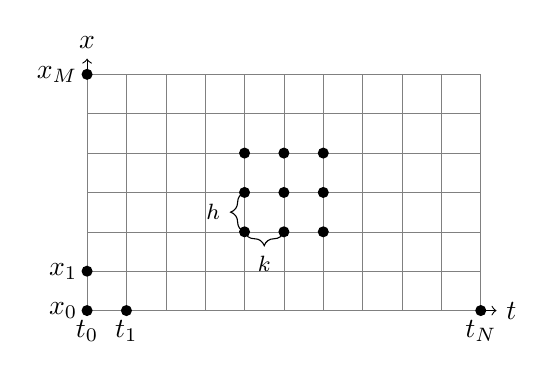
\begin{tikzpicture}

    % Axes
    \draw[->] (0,0) -- (5.2,0) node[right] {\(t\)};
    \draw[->] (0,0) -- (0,3.2) node[above] {\(x\)};

    % Grid points
    \draw[step=0.5cm,gray,very thin] (0,0) grid (5,3);

    \node[below] at (0,0) {\(t_0\)};
    \node[below] at (0.5,0) {\(t_1\)};
    \node[below] at (5,0) {\(t_N\)};
    \node[left] at (0,0) {\(x_0\)};
    \node[left] at (0,0.5) {\(x_1\)};
    \node[left] at (0,3) {\(x_M\)};

    % Add some key points with labels
    \foreach \x in {2,2.5,3} {
        \foreach \y in {1,1.5,2} {
            \fill (\x,\y) circle (2pt);
          }
      }

    % Add curly braces to show length k and h on axes
    \draw [decorate,decoration={brace,amplitude=5pt}]
    (2.5,1) -- (2,1) node [black,midway,yshift=-0.4cm] {\footnotesize \(k\)};
    \draw [decorate,decoration={brace,amplitude=5pt}]
    (2,1) -- (2,1.5) node [black,midway,xshift=-0.4cm] {\footnotesize \(h\)};

    % Add circles/points at nodes
    \fill (0,0) circle (2pt);
    \fill (0.5,0) circle (2pt);
    \fill (5,0) circle (2pt);
    \fill (0,0.5) circle (2pt);
    \fill (0,3) circle (2pt);

  \end{tikzpicture}
\end{center}

\begin{remark}{Constant Grid Spacing}{step_sizes}
  For simplicity, \(h\) and \(k\) are constant \( x_{m+1} = x_m + h,\quad t_{n+1} = t_n + k \).
\end{remark}

\section{Finite Difference Schemes}

Finite difference methods approximate differential equations by replacing them with a system of algebraic equations on the chosen grid.
The heat equation is often solved with these methods for their simplicity and computational efficiency.

\paragraph{The Forward-Time Central-Space (FTCS) scheme}

FTSC is a simple and widely used method for solving the heat equation.
It approximates the time derivative with a forward difference and the spatial derivative with a central difference.


\begin{align*}
  \frac{1}{k} \nabla_t U_m^{n+1} & = \frac{\mu}{h^2} \delta_x^2 U_m^{n+1} + f(U_m^n)                                              \\
  \nabla_t U_m^{n+1}             & = r \delta_x^2 U_m^{n+1} + k f(U_m^n), \quad r = \frac{\mu k}{h^2}                             \\
  U_m^{n+1}                      & = U_m^n + r \left( U_{m+1}^{n+1} - 2 U_m^{n+1} + U_{m-1}^{n+1} \right) + k f(U_m^n) \tag{FTCS}
\end{align*}

\paragraph{Crank-Nicolson Scheme}

The Crank-Nicolson scheme is an implicit method that approximates the spatial derivative at the midpoint between time steps. It is unconditionally stable and second-order accurate in time and space.
\begin{align*}
  U_m^\star & = U_m^n + \frac{r}{2} \left( \delta_x^2 U_m^\star + \delta_x^2 U_m^n \right) + k f(U_m^n), \quad r = \frac{\mu k}{h^2} \\
  U_m^{n+1} & = U_m^\star + \frac{k}{2} \left( f(U_m^\star) - f(U_m^n) \right) \tag{Crank-Nicolson}
\end{align*}

\section{Error Analysis}
Given the function \(f(u) = au\) for constant \(a\), we first want to analyze the consistency of the Crank-Nicolson scheme by determining the local truncation error (LTE).

\subsection{Consistency analysis (Local Truncation Error)}
The local truncation error (LTE) is the error at a single grid point when approximating a differential equation with a finite difference scheme.
It is the difference between the exact solution \(u(x_m, t_n)\) and the numerical approximation \(U_m^n\).

\begin{theorem}{Local truncation error for Crank-Nicolson}{thm:lte_cn}
  Consider the heat equation with linear reaction term \(f(u) = au\) for constant \(a\), discretized using the Crank-Nicolson scheme. Let \(u_m^n = u(x_m,t_n)\) denote the exact solution at grid points and \(u_m^\star = u(x_m, t_n + \Phi k)\) for \(\Phi \in [0,1]\) be an intermediate solution.

  The local truncation error \(\tau_m^n = \norm{u(x_m, t_n) - U_m^n}\) satisfies
  \[
    \norm{\tau_m^n} = \mathcal{O}(k + \tfrac{h^4}{k})
  \]
  When choosing the time step \(k \sim h^2\), the scheme achieves second-order accuracy in both time and space:
  \[
    \norm{\tau_m^n} = \mathcal{O}(h^2 + k^2)
  \]
\end{theorem}
\begin{proof}[Proof of Theorem~\ref{thm:lte_cn}]

  Denote
  \[
    u_m^n = u(x_m, t_n),
    \;
    u_m^\star = u\bigl(x_m,\, t_n + \Phi k\bigr), \quad \Phi \in [0, 1] \tag{Exact and intermediate solutions}
  \]

  We will use Taylor expansions around $(x_m, t_n)$ in both space and time~\ref{eq:taylor}.

  From central differences, we have
  \[
    \delta_x^2 u_m^n
    \;=\; u_{m+1}^n \;-\; 2\,u_m^n \;+\; u_{m-1}^n
    \;=\; h^2\,\partial_{xx}u_m^n \;+\; \mathcal{O}\bigl(h^4\bigr).
  \]
  Since $u_m^\star = u\bigl(x_m,\ t_n+\Phi k\bigr)$, similar Taylor expansions yield
  \[
    \delta_x^2 u_m^\star
    \;=\; u_{m+1}^\star \;-\; 2\,u_m^\star \;+\; u_{m-1}^\star
    \;=\; h^2\,\partial_{xx}u_m^n \;+\; \mathcal{O}\bigl(h^4 + k^4\bigr).
  \]

  Substitute these into the Crank--Nicolson half-step:
  \[
    U_m^\star
    \;=\; U_m^n
    \;+\; \frac{r}{2}\bigl(\delta_x^2 U_m^\star + \delta_x^2 U_m^n\bigr)
    \;+\; k\,a\,U_m^n,
    \quad
    r \;=\; \frac{\mu\,k}{h^2}.
  \]
  Matching $U_m^\star$ with the exact solution plus higher-order terms, we get
  \[
    U_m^\star
    \;=\; u_m^n
    \;+\; r\,h^2\,\partial_{xx}u_m^n
    \;+\; k\,a\,u_m^n
    \;+\; \mathcal{O}\bigl(h^4 + k^4\bigr).
  \]

  Next, we compute the full step using the intermediate solution:

  \[
    U_m^{n+1}
    \;=\; U_m^\star
    \;+\; \tfrac{k}{2}\,\bigl(a\,U_m^\star - a\,U_m^n\bigr).
  \]
  Expand $U_m^\star$ in time around $(x_m,t_n)$ and collect terms carefully:
  \[
    U_m^{n+1}
    \;=\; u_m^n
    \;+\; k\,\partial_t u_m^n
    \;+\; \tfrac{k^2}{2}\,\partial_t^2 u_m^n
    \;+\; \tfrac{k^3}{6}\,\partial_t^3 u_m^n
    \;+\; \tfrac{a\,r\,k}{2}\,h^2\,\partial_{xx} u_m^n
    \;+\; \tfrac{a^2\,k^2}{2}\,u_m^n
    \;+\; \mathcal{O}\bigl(k^4 + h^4\bigr).
  \]

  Since $r\,h^2 = \mu\,k$, the term involving $\partial_{xx} u_m^n$ can be written as
  $\tfrac{a\,\mu\,k^2}{2}\,\partial_{xx}u_m^n$.

  Compare to the exact solution at the next time level:

  \[
    u_m^{n+1}
    \;=\; u_m^n
    \;+\; k\,\partial_t u_m^n
    \;+\; \tfrac{k^2}{2}\,\partial_t^2 u_m^n
    \;+\; \tfrac{k^3}{6}\,\partial_t^3 u_m^n
    \;+\; \mathcal{O}\bigl(k^4\bigr).
  \]

  Their difference is
  \[
    U_m^{n+1} \;-\; u_m^{n+1}
    \;=\;
    \underbrace{\bigl(\tfrac{a\,\mu\,k^2}{2}\,\partial_{xx}u_m^n
      + \tfrac{a^2\,k^2}{2}\,u_m^n\bigr)}_{\mathcal{O}(k^2)}
    \;+\; \mathcal{O}\bigl(k^3 + h^4\bigr)
    \;=\; \mathcal{O}\bigl(k^2 + h^4\bigr).
  \]
  Thus, the local truncation error (per time step) is
  \[
    \lVert{\tau_m^n}\rVert
    \;=\; \left\lVert\dfrac{1}{k}\left(U_m^{n+1} - u_m^{n+1}\right) \right\rVert
    \;=\; \mathcal{O}\bigl(k + \tfrac{h^4}{k}\bigr).
  \]
  If we choose $k \sim h^2$, then
  \[
    \frac{h^4}{k} \;\sim\; h^2,
    \quad
    \Rightarrow
    \quad
    \lVert{\tau_m^n}\rVert \;\approx\; \mathcal{O}\bigl(k^2 + h^2\bigr).
  \]
  Therefore, under the usual choice $k \propto h^2$, the scheme is second-order accurate in both time and space.

\end{proof}




We denote the exact, and intermediate PDE solution by
\[
  u_m^n = u(x_m, t_n), \quad u_m^\star = u(x_m, t_n + \Phi k)
\]
Where \(\Phi \in [0, 1]\) is a parameter that interpolates between the time levels \(t_n\) and \(t_{n+1}\).

We want to find the local truncation error (LTE) of the Crank-Nicolson scheme, which is the error at a single grid point when approximating the PDE with the finite difference scheme.

\[
  \norm{\tau_m^n} = \norm{u(x_m, t_n) - U_m^n} = \mathcal{O}(h^p + k^q) \quad \text{as} \quad h, k \to 0
\]

Then we substitute these expansions into the finite difference schemes to analyze the local truncation error (LTE):

\begin{align*}
  \delta_x^2 u_m^n & = u_{m+1}^n - 2 u_m^n + u_{m-1}^n                                                                                                    \\
                   & = \left[ u_m^n + h \partial_x u_m^n + \frac{h^2}{2} \partial_x^2 u_m^n + \frac{h^3}{6} \partial_x^3 u_m^n + \mathcal{O}(h^4) \right] \\
                   & - 2 u_m^n                                                                                                                            \\
                   & + \left[ u_m^n - h \partial_x u_m^n + \frac{h^2}{2} \partial_x^2 u_m^n - \frac{h^3}{6} \partial_x^3 u_m^n + \mathcal{O}(h^4) \right] \\
                   & = h^2 \partial_x^2 u_m^n + \mathcal{O}(h^4)
\end{align*}

\begin{align*}
  \delta_x^2 u_m^\star & = u_{m+1}^\star - 2 u_m^\star + u_{m-1}^\star                                                                                                                                                                                                                                 \\
                       & = \left[ u_m^n + \left(\Phi k \partial_t u_m^n + h \partial_x u_m^n\right) + \frac{1}{2}\left(\Phi^2 k^2 \partial_t^2 u_m^n + h^2 \partial_x^2 u_m^n\right) + \frac{1}{6}\left(\Phi^3 k^3 \partial_t^3 u_m^n + h^3 \partial_x^3 u_m^n\right) + \mathcal{O}(h^4 + k^4) \right] \\
                       & - 2 \left[ u_m^n + \Phi k \partial_t u_m^n + \frac{(\Phi k)^2}{2} \partial_t^2 u_m^n + \frac{(\Phi k)^3}{6} \partial_t^3 u_m^n + \mathcal{O}(k^4) \right]                                                                                                                     \\
                       & + \left[ u_m^n + \left(\Phi k \partial_t u_m^n - h \partial_x u_m^n\right) + \frac{1}{2}\left(\Phi^2 k^2 \partial_t^2 u_m^n + h^2 \partial_x^2 u_m^n\right) + \frac{1}{6}\left(\Phi^3 k^3 \partial_t^3 u_m^n - h^3 \partial_x^3 u_m^n\right) + \mathcal{O}(h^4 + k^4) \right] \\
                       & = h^2 \partial_x^2 u_m^n + \mathcal{O}(h^4 + k^4)                                                                                                                                                                                                                             \\
\end{align*}

Then we substitute these expansions into the Crank-Nicolson scheme to analyze the local truncation error (LTE):
\begin{align*}
  U_m^\star & = U_m^n + \frac{r}{2} \left( \delta_x^2 U_m^\star + \delta_x^2 U_m^n \right) + k a U_m^n                                  \\
            & = u_m^n + \frac{r}{2} \left( h^2 \partial_x^2 u_m^n + h^2 \partial_x^2 u_m^n \right) + k a u_m^n + \mathcal{O}(h^4 + k^4) \\
            & = u_m^n + r h^2 \partial_x^2 u_m^n + k a u_m^n + \mathcal{O}(h^4 + k^4)                                                   \\
\end{align*}

By substituting the expansions into the Crank-Nicolson scheme, we can analyze the local truncation error (LTE) of the scheme.

\begin{align*}
  U_m^{n+1} & = U_m^\star + \tfrac{k}{2} \Bigl( a\,U_m^\star - a\,U_m^n \Bigr)                                                                            \\[1mm]
            & = \Bigl[ u_m^n + k\,\partial_t u_m^n + \tfrac{k^2}{2}\,\partial_t^2 u_m^n + \tfrac{k^3}{6}\,\partial_t^3 u_m^n + \mathcal{O}(k^4) \Bigr]    \\
            & \quad {}+ \tfrac{k\,a}{2}\Bigl\{ \Bigl[ u_m^n + r\,h^2\,\partial_{xx} u_m^n + k\,a\,u_m^n
  + \mathcal{O}(h^4+k^2) \Bigr] - u_m^n \Bigr\}                                                                                                           \\[1mm]
            & = u_m^n + k\,\partial_t u_m^n + \tfrac{k^2}{2}\,\partial_t^2 u_m^n
  + \tfrac{k^3}{6}\,\partial_t^3 u_m^n + \mathcal{O}(k^4) + \tfrac{k\,a}{2}\Bigl( r\,h^2\,\partial_{xx} u_m^n + k\,a\,u_m^n \Bigr) + \mathcal{O}(h^4+k^4) \\[1mm]
            & = u_m^n + k\,\partial_t u_m^n + \tfrac{k^2}{2}\,\partial_t^2 u_m^n
  + \tfrac{k^3}{6}\,\partial_t^3 u_m^n
  + \tfrac{a\,r\,k}{2}\,h^2\,\partial_{xx} u_m^n + \tfrac{a^2\,k^2}{2}\,u_m^n
  + \mathcal{O}(k^4+h^4)
\end{align*}

Using \(r=\frac{\mu k}{h^2}\) so that \(r\,h^2=\mu k\), we rewrite the above as
\begin{align*}
  U_m^{n+1} & = u_m^n + k\,\partial_t u_m^n + \tfrac{k^2}{2}\,\partial_t^2 u_m^n
  + \tfrac{k^3}{6}\,\partial_t^3 u_m^n
  + \tfrac{a\,\mu\,k^2}{2}\,\partial_{xx} u_m^n + \tfrac{a^2\,k^2}{2}\,u_m^n
  + \mathcal{O}(k^4+h^4).
\end{align*}

The left-hand side of the scheme is the exact solution at the next time level:
\begin{align*}
  u_m^{n+1}
   & = u_m^n + k\,\partial_t u_m^n + \tfrac{k^2}{2}\,\partial_t^2 u_m^n
  + \tfrac{k^3}{6}\,\partial_t^3 u_m^n + \mathcal{O}(k^4).
\end{align*}

The local truncation error (LTE) is the difference between the exact solution and the numerical approximation:

\begin{align*}
  U_m^{n+1} - u_m^{n+1} & =
  \left[ u_m^n + k\,\partial_t u_m^n + \tfrac{k^2}{2}\,\partial_t^2 u_m^n + \tfrac{k^3}{6}\,\partial_t^3 u_m^n + \mathcal{O}(k^4) \right]                                                            \\
                        & - \left[ u_m^n + k\,\mu\,\partial_{x}^2 u_m^n + k\,a\,u_m^n + \tfrac{a\,\mu\,k^2}{2}\,\partial_{x}^2 u_m^n + \tfrac{a^2\,k^2}{2}\,u_m^n \right] + \mathcal{O}(k^4+h^4)     \\
                        & = k^2 \left[\tfrac{1}{2}\partial_t^2 u_m^n - \tfrac{a \,\mu}{2}\partial_{x}^2 u_m^n - \tfrac{a^2}{2}u_m^n\right] + \tfrac{k^3}{6}\partial_t^3 u_m^n + \mathcal{O}(k^4+h^4) \\
                        & = \mathcal{O}(k^2 + h^4)                                                                                                                                                   \\[2mm]
  \norm{\tau_m^n}       & = \norm{\frac{U_m^{n+1} - u_m^{n+1}}{k}} = \mathcal{O}(k + \frac{h^4}{k})                                                                                                  \\
\end{align*}

If we choose time step \(k\) such that \(k \sim h^2\) is of similar order as the spatial step, then the LTE is a second-order error in both time and space:

\begin{equation}
  \norm{\tau_m^n} = \mathcal{O}(k + \frac{h^4}{k}) \approx \mathcal{O}(k^2 + h^2) \quad \text{where} \quad k \sim h^2
\end{equation}

\subsection{Stability Analysis (Von Neumann Stability)}
The Von Neumann stability analysis is a method to determine the stability of a finite difference scheme by analyzing the growth of errors in the Fourier modes of the solution.

\begin{theorem}{Stability of the Crank-Nicolson scheme}{stability_cn}
  The Crank-Nicolson scheme is stable for the heat equation with linear reaction term \(f(u) = au\) for constant \(a\) if the time step \(k\) satisfies the condition
  \[
    k \leq \frac{h^2}{2\mu} \quad \text{where} \quad r = \frac{\mu k}{h^2}
  \]
  and the amplification factor \(\xi\) satisfies
  \[
    \norm{\xi} \leq 1 + Ck
  \]
\end{theorem}
\begin{proof}[Proof of Theorem~\ref{thm:stability_cn}]
  Let \(U_m^n = \xi^n e^{i m \theta}\) be the Fourier mode of the numerical solution at grid point \((x_m, t_n)\), where \(\xi\) is the amplification factor and \(\theta\) is the wave number.
  For the first step of the Crank-Nicolson scheme, we substitute the Fourier mode and the reaction term \(f(u) = au\):

  \begin{align*}
    U_m^\star                & = U_m^n + \frac{r}{2} (\delta_x^2 U_m^\star + \delta_x^2 U_m^n) + k a U_m^n                                                                          \\
    \xi^\star e^{i m \theta} & = \xi^n e^{i m \theta} + \frac{r}{2} \left(\xi^\star + \xi^n\right)\left(e^{i\theta} - 2 + e^{-i\theta}\right)e^{im\theta}+ k a \xi^n e^{i m \theta} \\
    \xi^\star                & = \xi^n + \frac{r}{2} \left(\xi^\star + \xi^n \right)\overbrace{\left(e^{i \theta} - 2 + e^{-i \theta}\right)}^{2\cos\theta - 2} + k a \xi^n                                       \\
    \xi^\star                & = (1 + r(\cos(\theta) - 1) + ka) \xi^n + r(\cos(\theta) - 1)\xi^\star                                                                                \\
    \xi^\star                & = \frac{(1 + ka) + r(\cos(\theta) - 1)}{1 - r(\cos(\theta) - 1)} \xi^n                                                                               \\
  \end{align*}

  For the second step, substitute the Fourier mode into the Crank-Nicolson scheme:

  \begin{align*}
    U_m^{n+1}                & = U_m^\star + \frac{k}{2}(a U_m^\star - a U_m^n)                                                                        \\
    \xi^{n+1} e^{i m \theta} & = \xi^\star e^{i m \theta} + \frac{ka}{2}(\xi^\star - \xi^n)e^{i m \theta}                                              \\
    \xi^{n+1}                & = (1 + \frac{ka}{2}) \xi^\star - \frac{ka}{2} \xi^n                                                                     \\
    \frac{\xi^{n+1}}{\xi^n}  & = -\frac{{ak}^2 + 2(a k + 1) (r (\cos(\theta) - 1) + 1)}{2 (r (\cos(\theta) - 1) - 1)}       \tag{Source: Trust me bro} \\
  \end{align*}

  Let \(\beta = r(\cos(\theta) - 1)\) and \(\alpha = ka\), then we have the amplification factor \(\xi=\frac{\xi^{n+1}}{\xi^n}\):

  \[
    \xi = -\frac{\alpha^2 + 2(\alpha + 1)(\beta + 1)}{2(\beta - 1)}
  \]

  Furthermore, we can now find a bound for the amplification factor:

  \begin{align*}
    \norm*{\xi}                                                       & \leq 1 + Ck                                                                                                                                                    \\
    \norm*{-\frac{\alpha^2 + 2(\alpha + 1)(\beta + 1)}{2(\beta - 1)}} & = \norm*{\frac{\alpha^2 + 2(\alpha + 1)(\beta + 1)}{2(\beta - 1)}}                                                                                             \\
                                                                      & \leq \norm*{\frac{\alpha^2}{2(\beta - 1)}} + \norm*{\frac{(\alpha + 1)(\beta + 1)}{2(\beta - 1)}}                                                              \\
                                                                      & \leq \frac{\alpha^2}{2\underbrace{\abs{\beta - 1}}_{\geq 1}} + \frac{(\alpha + 1)\overbrace{\abs{\beta + 1}}^{\leq 1}}{2\underbrace{\abs{\beta - 1}}_{\geq 1}} \\
  \end{align*}
\end{proof}


